\documentclass[a4paper,11pt]{report}
\usepackage{amssymb}
\usepackage{epsfig}

\author{Tommy Petersen}

\title{User's manual to the suffix tree}

\begin{document}

\maketitle

\newcommand{\R}{\mathbb{R}}
\newcommand{\Q}{\mathbb{Q}}
\newcommand{\Z}{\mathbb{Z}}
\newcommand{\N}{\mathbb{N}}

\newtheorem{lemma}{Lemma}[section]
\newtheorem{proposition}{Proposition}[section]
\newtheorem{theorem}{Theorem}[section]
\newtheorem{corollary}{Corollary}[section]
\newtheorem{algorithm}{Algorithm}[section]
\newtheorem{definition}{Definition}[section]
\newtheorem{example}{Example}[section]

\copyright{ AI Agents 2005}

\tableofcontents

\chapter{User's manual}
\section{Preface}
This is an incomplete edition of the user's manual to the java suffix tree implementation
by AI Agents. Still, it is published, because it contains useful information to the users.
I expect that the readers know how to compile and run java programs grouped in packages.
If you have questions or suggestions for additions to the manual, then write me at tp@ai-agents.com.

\section{Context}
A context of a given string $s$ is a suffix of $s$ that has occured earlier as a substring of $s$.
An example is the string $s := 0110100110101101$. The largest context is the suffix $01101$.
Every other suffix, including the empty context, $\lambda$, of this largest context is also a context
in $s$.

If a context has only one preceding substring it is said to have decoded a suffix, because only one
suffix can follow as a future sequence when trusting what has been learned. On the other hand, if
the context has more than one preceding substring, then there is more than one possibility for the
future sequence, when using what has been learned. In the above example with $s$ equal to the sequence
$0110100110101101$, none of the contexts decode a suffix. But with $s := 010101$, the largest context
is $0101$ and the context set is $\{\lambda, 1, 01, 101, 0101\}$. The contexts $0101$ and $101$ both
decode a suffix, while the other three contexts do not decode a suffix.

In the java implementation, a context, {\it Context}, is given by a {\it baseVertex}, a {\it direction}
and an {\it offset}. The {\it baseVertex} is a vertex in the suffix tree, the {\it direction} tells
which direction to branch away from {\it baseVertex}, while the {\it offset} tells how many steps to take
along the branch. If {\it direction} equals $-1$ then the context points at the {\it baseVertex} implying
that no suffix is decoded and that if you use the {\it indexTo} from {\it baseVertex} then you get an
index, $i$, where $s[i]$ is identical to the last symbol in the context. Note, that {\it indexTo} equals
infinity when the vertex containing it is a leaf. If {\it direction} is greater
than $-1$, then the context points at the edge extending from {\it baseVertex} in direction
{\it direction}. If you use the index $i:=$ {\it baseVertex}.{\it indexFrom}$[${\it direction}$] + $
{\it offset}, then $s[i]$ is identical to the last symbol in the context. Note, that if {\it direction}
is greater than $-1$ and {\it baseVertex}.{\it child}$[${\it direction}$]$ is a leaf, then the context
decodes a suffix, and the symbol $s[i+1]$ should be the next symbol in the future sequence, if one can
trust what has been learned about this particular context. Figure~\ref{fig:contexts} illustrates the
possible types of contexts.
\begin{figure}
  \centering
  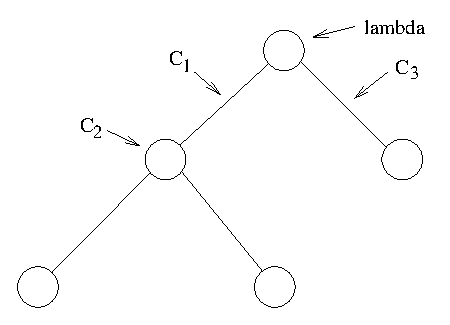
\epsfig{file=Eps/contexts.eps}
  \caption{All possible types of contexts. The context $\lambda$ is always in the context set. The
  contexts $C_1, C_2$ and $C_3$ are not necessarily in the same context set. For $C_1$, {\it direction}
  is greater than $-1$, but $C_1$ does not decode a suffix. For $C_2$, {\it direction} equals $-1$.
  Finally, for $C_3$, {\it direction} is greater than $-1$ and $C_3$ decodes a suffix.}
  \label{fig:contexts}
\end{figure}
Also note, that a leaf can never be the base vertex of any context.

The string $s$ can be retrieved by calling the method {\it getL} from any given context.


In the java implementation, a set of contexts, {\it contextSet}, is returned each time a new symbol
is added to the suffix tree.

\section{Average copy length}
\begin{definition}[Copy length for a context]
The copy length for a given context $C$ is the sum of the length of all suffixes immediately following instances of $C$ in
the code word set. Note, that this omits suffixes in the context set.
\end{definition}
\begin{definition}[Number of leaves for a context]
 The number of leaves for a given context $C$ is the number of leaves in the subtree rooted in either $C$'s basevertex 
(if this basevertex has no direction or the child in the direction is a leaf) or its child (if the basevertex has a
direction and the child in that direction is not a leaf).
\end{definition}
\begin{definition}[Average copy length for a context]
The average copy length for a given context $C$ equals the quotient of the copy length for the context to the
number of leaves for the context.
\end{definition}
\begin{example}[Average copy length for a context]
Let $L$ be the sequence $011010011010$. The context set is then $\{\lambda, 0, 10, 010, 1010, 11010, 011010\}$, and
the code word set is $\{011, 11, 101, 010, 100, 00\}$. The suffix tree is shown in figure~\ref{fig:stree1}
\end{example}
\begin{figure}
  \centering
  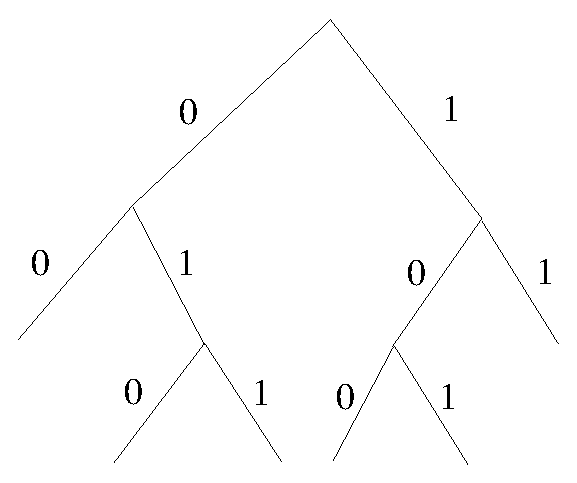
\epsfig{file=Eps/stree1.eps}
  \caption{The suffix tree for the sequence $011010011010$.}
  \label{fig:stree1}
\end{figure}
\begin{center}
\begin{tabular}{|l|r|r|r|} \hline
Context   & Copy length                     & \#leaves & Average copy length \\ \hline
$\lambda$ & $12 + 11 + 10 + 9 + 8 + 7 = 57$ & $6$     & $9.5   $            \\ \hline
$0$       & $11 + 8 + 6 = 25$               & $3$     & $8.3334$            \\ \hline
$10$      & $8 + 6 = 14$                    & $2$     & $7     $            \\ \hline
$010$     & $6$                             & $1$     & $6     $            \\ \hline
$1010$    & $6$                             & $1$     & $6     $            \\ \hline
$11010$   & $6$                             & $1$     & $6     $            \\ \hline
$011010$  & $6$                             & $1$     & $6     $            \\ \hline
\end{tabular}
\end{center}
Note, that suffixes in the context set are omitted when computing the copy lengths. For example,
the shortest copy length instance for the context $\lambda$ is $7$ even though $\lambda$ is a prefix
of every suffix in the sequence $L$.

\chapter{The java implementation}
\section{Source files}
The package name is {\sl AIAgents.SuffixTree.Java} and the source files are listed here:
\begin{itemize}
\item {\sl Context.java}
\item {\sl Vertex.java}
\item {\sl codeWordSet.java}
\item {\sl contextSet.java}
\item {\sl suffixTree.java}
\item {\sl test.java}
\end{itemize}
{\sl test.java} is not necessary in the implementation, but you can look in it in order to see how to
use the suffix tree.


\end{document}
